
%(BEGIN_QUESTION)
% Copyright 2014, Tony R. Kuphaldt, released under the Creative Commons Attribution License (v 1.0)
% This means you may do almost anything with this work of mine, so long as you give me proper credit

Regn ut resistansen til strekklappen i denne målebro-kretsen, gitt voltmeterets indikasjon på 5.6 mV (A er positiv og B er negativ).

$$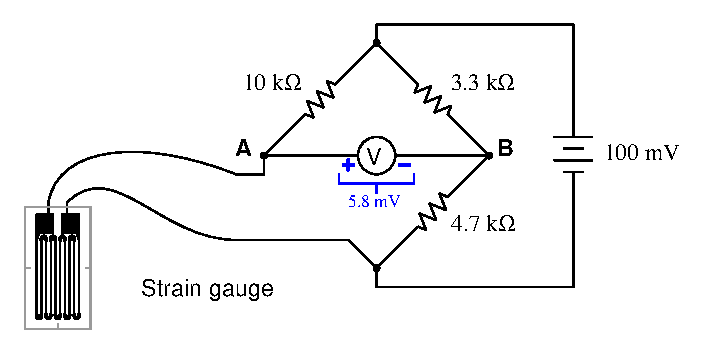
\includegraphics[width=15.5cm]{i00854x01.eps}$$

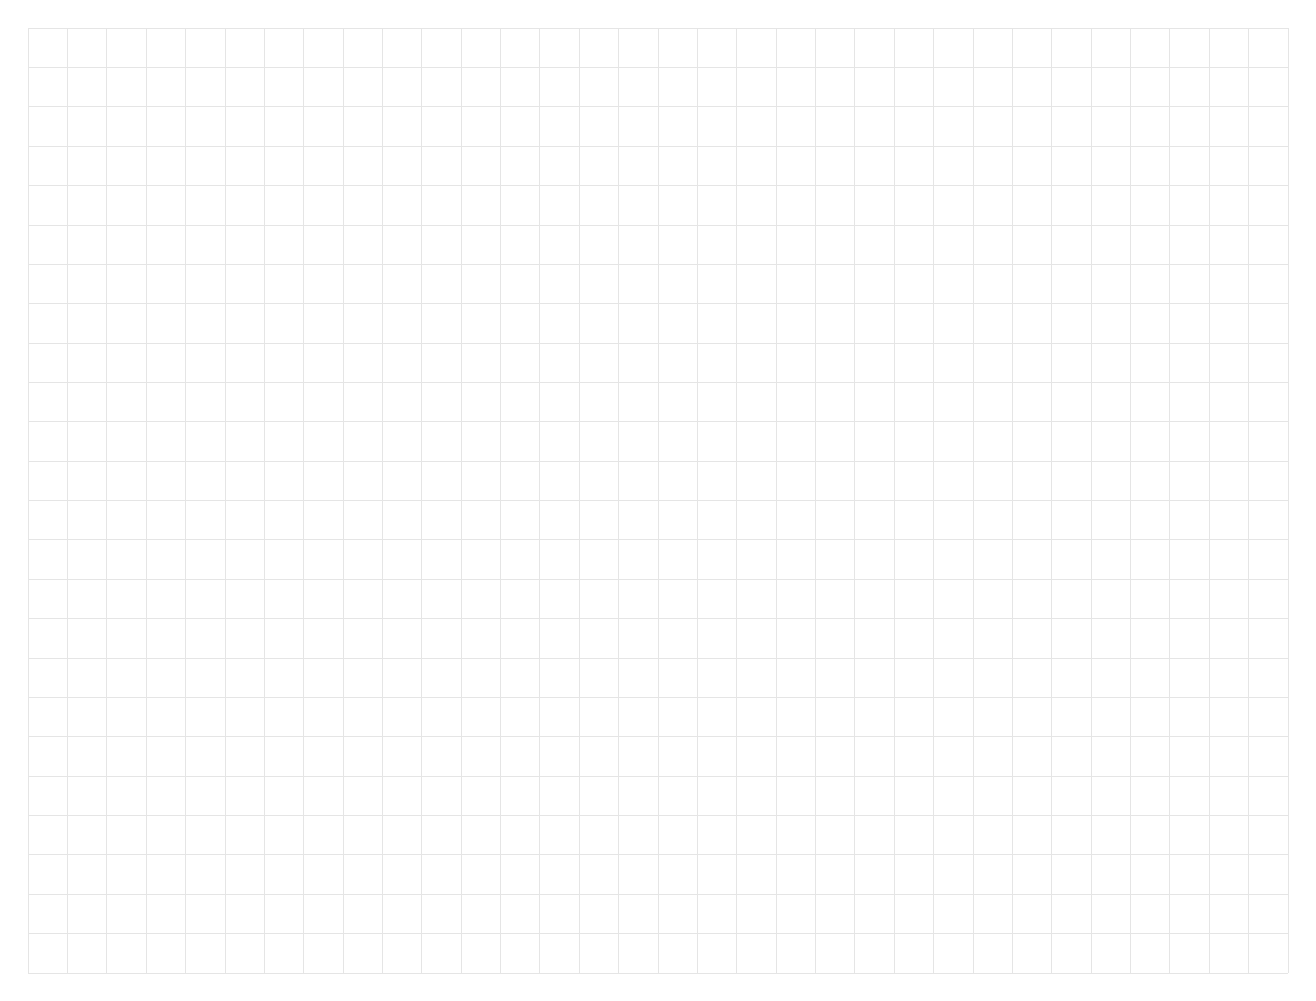
\begin{tikzpicture}
	\draw[step=0.5cm,gray!20,very thin]  grid (16,12) ;
\end{tikzpicture}
$R_{strain}$ = \underbar{\hskip 50pt}

\vfil 

\underbar{file i00854}
\eject
%(END_QUESTION)





%(BEGIN_ANSWER)

Dette er en vurdert oppgave -- ingen svar eller hint oppgis!

%(END_ANSWER)





%(BEGIN_NOTES)

Voltmeterets indikasjon på 5.8 mV (der A er mer positiv enn B) forteller oss at strekklappen har så mye større spenningsfall enn 4.7 k$\Omega$-motstanden. Strategien blir derfor først å beregne spenningsfallet over 4.7 k$\Omega$-motstanden, deretter legge til 5.8 mV, og til slutt beregne $R_{strain}$.

\vskip 10pt

Først: spenningsfall over 4.7 k$\Omega$-motstanden:

$$V_{4.7k} = 100 \hbox{ mV} \left(4700 \> \Omega \over {3300 \> \Omega + 4700 \> \Omega}\right) = 58.75 \hbox{ mV}$$

Nå: spenningsfall over strekklappen:

$$V_{strain} = 58.75 \hbox{ mV} + 5.8 \hbox{ mV} = 64.55 \hbox{ mV}$$

Når strekklappen har 64.55 mV spenningsfall, må 10 k$\Omega$-motstanden ta resten av de 100 mV (Kirchhoffs spenningslov):

$$V_{10k} = 100 \hbox{ mV} - 64.55 \hbox{ mV} = 35.45 \hbox{ mV}$$

Ohms lov gir strømmen gjennom 10 k$\Omega$-motstanden, som også er samme strøm gjennom strekklappen:

$$I = {V \over R} = {35.45 \hbox{ mV} \over 10000 \> \Omega} = 3.545 \> \mu\hbox{A}$$

Nå kjenner vi både strøm gjennom strekklappen (3.545 $\mu$A) og spenning over den (64.55 mV), og kan bruke Ohms lov for motstanden:

$$R_{strain} = {V \over I} = {64.55 \hbox{ mV} \over 3.545 \> \mu\hbox{A}} = 18.21 \hbox{ k}\Omega$$

%INDEX% Electronics review: Kirchhoff's Voltage Law (KVL)
%INDEX% Electronics review: series-parallel circuits
%INDEX% Measurement, strain gauge

%(END_NOTES)
